\documentclass{article}
\PassOptionsToPackage{table}{xcolor}
\usepackage{iclr2027_conference,times}
\iclrfinalcopy
%%%%% NEW MATH DEFINITIONS %%%%%

\usepackage{amsmath,amsfonts,bm}

% Mark sections of captions for referring to divisions of figures
\newcommand{\figleft}{{\em (Left)}}
\newcommand{\figcenter}{{\em (Center)}}
\newcommand{\figright}{{\em (Right)}}
\newcommand{\figtop}{{\em (Top)}}
\newcommand{\figbottom}{{\em (Bottom)}}
\newcommand{\captiona}{{\em (a)}}
\newcommand{\captionb}{{\em (b)}}
\newcommand{\captionc}{{\em (c)}}
\newcommand{\captiond}{{\em (d)}}

% Highlight a newly defined term
\newcommand{\newterm}[1]{{\bf #1}}


% Figure reference, lower-case.
\def\figref#1{figure~\ref{#1}}
% Figure reference, capital. For start of sentence
\def\Figref#1{Figure~\ref{#1}}
\def\twofigref#1#2{figures \ref{#1} and \ref{#2}}
\def\quadfigref#1#2#3#4{figures \ref{#1}, \ref{#2}, \ref{#3} and \ref{#4}}
% Section reference, lower-case.
\def\secref#1{section~\ref{#1}}
% Section reference, capital.
\def\Secref#1{Section~\ref{#1}}
% Reference to two sections.
\def\twosecrefs#1#2{sections \ref{#1} and \ref{#2}}
% Reference to three sections.
\def\secrefs#1#2#3{sections \ref{#1}, \ref{#2} and \ref{#3}}
% Reference to an equation, lower-case.
\def\eqref#1{equation~\ref{#1}}
% Reference to an equation, upper case
\def\Eqref#1{Equation~\ref{#1}}
% A raw reference to an equation---avoid using if possible
\def\plaineqref#1{\ref{#1}}
% Reference to a chapter, lower-case.
\def\chapref#1{chapter~\ref{#1}}
% Reference to an equation, upper case.
\def\Chapref#1{Chapter~\ref{#1}}
% Reference to a range of chapters
\def\rangechapref#1#2{chapters\ref{#1}--\ref{#2}}
% Reference to an algorithm, lower-case.
\def\algref#1{algorithm~\ref{#1}}
% Reference to an algorithm, upper case.
\def\Algref#1{Algorithm~\ref{#1}}
\def\twoalgref#1#2{algorithms \ref{#1} and \ref{#2}}
\def\Twoalgref#1#2{Algorithms \ref{#1} and \ref{#2}}
% Reference to a part, lower case
\def\partref#1{part~\ref{#1}}
% Reference to a part, upper case
\def\Partref#1{Part~\ref{#1}}
\def\twopartref#1#2{parts \ref{#1} and \ref{#2}}

\def\ceil#1{\lceil #1 \rceil}
\def\floor#1{\lfloor #1 \rfloor}
\def\1{\bm{1}}
\newcommand{\train}{\mathcal{D}}
\newcommand{\valid}{\mathcal{D_{\mathrm{valid}}}}
\newcommand{\test}{\mathcal{D_{\mathrm{test}}}}

\def\eps{{\epsilon}}


% Random variables
\def\reta{{\textnormal{$\eta$}}}
\def\ra{{\textnormal{a}}}
\def\rb{{\textnormal{b}}}
\def\rc{{\textnormal{c}}}
\def\rd{{\textnormal{d}}}
\def\re{{\textnormal{e}}}
\def\rf{{\textnormal{f}}}
\def\rg{{\textnormal{g}}}
\def\rh{{\textnormal{h}}}
\def\ri{{\textnormal{i}}}
\def\rj{{\textnormal{j}}}
\def\rk{{\textnormal{k}}}
\def\rl{{\textnormal{l}}}
% rm is already a command, just don't name any random variables m
\def\rn{{\textnormal{n}}}
\def\ro{{\textnormal{o}}}
\def\rp{{\textnormal{p}}}
\def\rq{{\textnormal{q}}}
\def\rr{{\textnormal{r}}}
\def\rs{{\textnormal{s}}}
\def\rt{{\textnormal{t}}}
\def\ru{{\textnormal{u}}}
\def\rv{{\textnormal{v}}}
\def\rw{{\textnormal{w}}}
\def\rx{{\textnormal{x}}}
\def\ry{{\textnormal{y}}}
\def\rz{{\textnormal{z}}}

% Random vectors
\def\rvepsilon{{\mathbf{\epsilon}}}
\def\rvtheta{{\mathbf{\theta}}}
\def\rva{{\mathbf{a}}}
\def\rvb{{\mathbf{b}}}
\def\rvc{{\mathbf{c}}}
\def\rvd{{\mathbf{d}}}
\def\rve{{\mathbf{e}}}
\def\rvf{{\mathbf{f}}}
\def\rvg{{\mathbf{g}}}
\def\rvh{{\mathbf{h}}}
\def\rvu{{\mathbf{i}}}
\def\rvj{{\mathbf{j}}}
\def\rvk{{\mathbf{k}}}
\def\rvl{{\mathbf{l}}}
\def\rvm{{\mathbf{m}}}
\def\rvn{{\mathbf{n}}}
\def\rvo{{\mathbf{o}}}
\def\rvp{{\mathbf{p}}}
\def\rvq{{\mathbf{q}}}
\def\rvr{{\mathbf{r}}}
\def\rvs{{\mathbf{s}}}
\def\rvt{{\mathbf{t}}}
\def\rvu{{\mathbf{u}}}
\def\rvv{{\mathbf{v}}}
\def\rvw{{\mathbf{w}}}
\def\rvx{{\mathbf{x}}}
\def\rvy{{\mathbf{y}}}
\def\rvz{{\mathbf{z}}}

% Elements of random vectors
\def\erva{{\textnormal{a}}}
\def\ervb{{\textnormal{b}}}
\def\ervc{{\textnormal{c}}}
\def\ervd{{\textnormal{d}}}
\def\erve{{\textnormal{e}}}
\def\ervf{{\textnormal{f}}}
\def\ervg{{\textnormal{g}}}
\def\ervh{{\textnormal{h}}}
\def\ervi{{\textnormal{i}}}
\def\ervj{{\textnormal{j}}}
\def\ervk{{\textnormal{k}}}
\def\ervl{{\textnormal{l}}}
\def\ervm{{\textnormal{m}}}
\def\ervn{{\textnormal{n}}}
\def\ervo{{\textnormal{o}}}
\def\ervp{{\textnormal{p}}}
\def\ervq{{\textnormal{q}}}
\def\ervr{{\textnormal{r}}}
\def\ervs{{\textnormal{s}}}
\def\ervt{{\textnormal{t}}}
\def\ervu{{\textnormal{u}}}
\def\ervv{{\textnormal{v}}}
\def\ervw{{\textnormal{w}}}
\def\ervx{{\textnormal{x}}}
\def\ervy{{\textnormal{y}}}
\def\ervz{{\textnormal{z}}}

% Random matrices
\def\rmA{{\mathbf{A}}}
\def\rmB{{\mathbf{B}}}
\def\rmC{{\mathbf{C}}}
\def\rmD{{\mathbf{D}}}
\def\rmE{{\mathbf{E}}}
\def\rmF{{\mathbf{F}}}
\def\rmG{{\mathbf{G}}}
\def\rmH{{\mathbf{H}}}
\def\rmI{{\mathbf{I}}}
\def\rmJ{{\mathbf{J}}}
\def\rmK{{\mathbf{K}}}
\def\rmL{{\mathbf{L}}}
\def\rmM{{\mathbf{M}}}
\def\rmN{{\mathbf{N}}}
\def\rmO{{\mathbf{O}}}
\def\rmP{{\mathbf{P}}}
\def\rmQ{{\mathbf{Q}}}
\def\rmR{{\mathbf{R}}}
\def\rmS{{\mathbf{S}}}
\def\rmT{{\mathbf{T}}}
\def\rmU{{\mathbf{U}}}
\def\rmV{{\mathbf{V}}}
\def\rmW{{\mathbf{W}}}
\def\rmX{{\mathbf{X}}}
\def\rmY{{\mathbf{Y}}}
\def\rmZ{{\mathbf{Z}}}

% Elements of random matrices
\def\ermA{{\textnormal{A}}}
\def\ermB{{\textnormal{B}}}
\def\ermC{{\textnormal{C}}}
\def\ermD{{\textnormal{D}}}
\def\ermE{{\textnormal{E}}}
\def\ermF{{\textnormal{F}}}
\def\ermG{{\textnormal{G}}}
\def\ermH{{\textnormal{H}}}
\def\ermI{{\textnormal{I}}}
\def\ermJ{{\textnormal{J}}}
\def\ermK{{\textnormal{K}}}
\def\ermL{{\textnormal{L}}}
\def\ermM{{\textnormal{M}}}
\def\ermN{{\textnormal{N}}}
\def\ermO{{\textnormal{O}}}
\def\ermP{{\textnormal{P}}}
\def\ermQ{{\textnormal{Q}}}
\def\ermR{{\textnormal{R}}}
\def\ermS{{\textnormal{S}}}
\def\ermT{{\textnormal{T}}}
\def\ermU{{\textnormal{U}}}
\def\ermV{{\textnormal{V}}}
\def\ermW{{\textnormal{W}}}
\def\ermX{{\textnormal{X}}}
\def\ermY{{\textnormal{Y}}}
\def\ermZ{{\textnormal{Z}}}

% Vectors
\def\vzero{{\bm{0}}}
\def\vone{{\bm{1}}}
\def\vmu{{\bm{\mu}}}
\def\vtheta{{\bm{\theta}}}
\def\va{{\bm{a}}}
\def\vb{{\bm{b}}}
\def\vc{{\bm{c}}}
\def\vd{{\bm{d}}}
\def\ve{{\bm{e}}}
\def\vf{{\bm{f}}}
\def\vg{{\bm{g}}}
\def\vh{{\bm{h}}}
\def\vi{{\bm{i}}}
\def\vj{{\bm{j}}}
\def\vk{{\bm{k}}}
\def\vl{{\bm{l}}}
\def\vm{{\bm{m}}}
\def\vn{{\bm{n}}}
\def\vo{{\bm{o}}}
\def\vp{{\bm{p}}}
\def\vq{{\bm{q}}}
\def\vr{{\bm{r}}}
\def\vs{{\bm{s}}}
\def\vt{{\bm{t}}}
\def\vu{{\bm{u}}}
\def\vv{{\bm{v}}}
\def\vw{{\bm{w}}}
\def\vx{{\bm{x}}}
\def\vy{{\bm{y}}}
\def\vz{{\bm{z}}}

% Elements of vectors
\def\evalpha{{\alpha}}
\def\evbeta{{\beta}}
\def\evepsilon{{\epsilon}}
\def\evlambda{{\lambda}}
\def\evomega{{\omega}}
\def\evmu{{\mu}}
\def\evpsi{{\psi}}
\def\evsigma{{\sigma}}
\def\evtheta{{\theta}}
\def\eva{{a}}
\def\evb{{b}}
\def\evc{{c}}
\def\evd{{d}}
\def\eve{{e}}
\def\evf{{f}}
\def\evg{{g}}
\def\evh{{h}}
\def\evi{{i}}
\def\evj{{j}}
\def\evk{{k}}
\def\evl{{l}}
\def\evm{{m}}
\def\evn{{n}}
\def\evo{{o}}
\def\evp{{p}}
\def\evq{{q}}
\def\evr{{r}}
\def\evs{{s}}
\def\evt{{t}}
\def\evu{{u}}
\def\evv{{v}}
\def\evw{{w}}
\def\evx{{x}}
\def\evy{{y}}
\def\evz{{z}}

% Matrix
\def\mA{{\bm{A}}}
\def\mB{{\bm{B}}}
\def\mC{{\bm{C}}}
\def\mD{{\bm{D}}}
\def\mE{{\bm{E}}}
\def\mF{{\bm{F}}}
\def\mG{{\bm{G}}}
\def\mH{{\bm{H}}}
\def\mI{{\bm{I}}}
\def\mJ{{\bm{J}}}
\def\mK{{\bm{K}}}
\def\mL{{\bm{L}}}
\def\mM{{\bm{M}}}
\def\mN{{\bm{N}}}
\def\mO{{\bm{O}}}
\def\mP{{\bm{P}}}
\def\mQ{{\bm{Q}}}
\def\mR{{\bm{R}}}
\def\mS{{\bm{S}}}
\def\mT{{\bm{T}}}
\def\mU{{\bm{U}}}
\def\mV{{\bm{V}}}
\def\mW{{\bm{W}}}
\def\mX{{\bm{X}}}
\def\mY{{\bm{Y}}}
\def\mZ{{\bm{Z}}}
\def\mBeta{{\bm{\beta}}}
\def\mPhi{{\bm{\Phi}}}
\def\mLambda{{\bm{\Lambda}}}
\def\mSigma{{\bm{\Sigma}}}

% Tensor
\DeclareMathAlphabet{\mathsfit}{\encodingdefault}{\sfdefault}{m}{sl}
\SetMathAlphabet{\mathsfit}{bold}{\encodingdefault}{\sfdefault}{bx}{n}
\newcommand{\tens}[1]{\bm{\mathsfit{#1}}}
\def\tA{{\tens{A}}}
\def\tB{{\tens{B}}}
\def\tC{{\tens{C}}}
\def\tD{{\tens{D}}}
\def\tE{{\tens{E}}}
\def\tF{{\tens{F}}}
\def\tG{{\tens{G}}}
\def\tH{{\tens{H}}}
\def\tI{{\tens{I}}}
\def\tJ{{\tens{J}}}
\def\tK{{\tens{K}}}
\def\tL{{\tens{L}}}
\def\tM{{\tens{M}}}
\def\tN{{\tens{N}}}
\def\tO{{\tens{O}}}
\def\tP{{\tens{P}}}
\def\tQ{{\tens{Q}}}
\def\tR{{\tens{R}}}
\def\tS{{\tens{S}}}
\def\tT{{\tens{T}}}
\def\tU{{\tens{U}}}
\def\tV{{\tens{V}}}
\def\tW{{\tens{W}}}
\def\tX{{\tens{X}}}
\def\tY{{\tens{Y}}}
\def\tZ{{\tens{Z}}}


% Graph
\def\gA{{\mathcal{A}}}
\def\gB{{\mathcal{B}}}
\def\gC{{\mathcal{C}}}
\def\gD{{\mathcal{D}}}
\def\gE{{\mathcal{E}}}
\def\gF{{\mathcal{F}}}
\def\gG{{\mathcal{G}}}
\def\gH{{\mathcal{H}}}
\def\gI{{\mathcal{I}}}
\def\gJ{{\mathcal{J}}}
\def\gK{{\mathcal{K}}}
\def\gL{{\mathcal{L}}}
\def\gM{{\mathcal{M}}}
\def\gN{{\mathcal{N}}}
\def\gO{{\mathcal{O}}}
\def\gP{{\mathcal{P}}}
\def\gQ{{\mathcal{Q}}}
\def\gR{{\mathcal{R}}}
\def\gS{{\mathcal{S}}}
\def\gT{{\mathcal{T}}}
\def\gU{{\mathcal{U}}}
\def\gV{{\mathcal{V}}}
\def\gW{{\mathcal{W}}}
\def\gX{{\mathcal{X}}}
\def\gY{{\mathcal{Y}}}
\def\gZ{{\mathcal{Z}}}

% Sets
\def\sA{{\mathbb{A}}}
\def\sB{{\mathbb{B}}}
\def\sC{{\mathbb{C}}}
\def\sD{{\mathbb{D}}}
% Don't use a set called E, because this would be the same as our symbol
% for expectation.
\def\sF{{\mathbb{F}}}
\def\sG{{\mathbb{G}}}
\def\sH{{\mathbb{H}}}
\def\sI{{\mathbb{I}}}
\def\sJ{{\mathbb{J}}}
\def\sK{{\mathbb{K}}}
\def\sL{{\mathbb{L}}}
\def\sM{{\mathbb{M}}}
\def\sN{{\mathbb{N}}}
\def\sO{{\mathbb{O}}}
\def\sP{{\mathbb{P}}}
\def\sQ{{\mathbb{Q}}}
\def\sR{{\mathbb{R}}}
\def\sS{{\mathbb{S}}}
\def\sT{{\mathbb{T}}}
\def\sU{{\mathbb{U}}}
\def\sV{{\mathbb{V}}}
\def\sW{{\mathbb{W}}}
\def\sX{{\mathbb{X}}}
\def\sY{{\mathbb{Y}}}
\def\sZ{{\mathbb{Z}}}

% Entries of a matrix
\def\emLambda{{\Lambda}}
\def\emA{{A}}
\def\emB{{B}}
\def\emC{{C}}
\def\emD{{D}}
\def\emE{{E}}
\def\emF{{F}}
\def\emG{{G}}
\def\emH{{H}}
\def\emI{{I}}
\def\emJ{{J}}
\def\emK{{K}}
\def\emL{{L}}
\def\emM{{M}}
\def\emN{{N}}
\def\emO{{O}}
\def\emP{{P}}
\def\emQ{{Q}}
\def\emR{{R}}
\def\emS{{S}}
\def\emT{{T}}
\def\emU{{U}}
\def\emV{{V}}
\def\emW{{W}}
\def\emX{{X}}
\def\emY{{Y}}
\def\emZ{{Z}}
\def\emSigma{{\Sigma}}

% entries of a tensor
% Same font as tensor, without \bm wrapper
\newcommand{\etens}[1]{\mathsfit{#1}}
\def\etLambda{{\etens{\Lambda}}}
\def\etA{{\etens{A}}}
\def\etB{{\etens{B}}}
\def\etC{{\etens{C}}}
\def\etD{{\etens{D}}}
\def\etE{{\etens{E}}}
\def\etF{{\etens{F}}}
\def\etG{{\etens{G}}}
\def\etH{{\etens{H}}}
\def\etI{{\etens{I}}}
\def\etJ{{\etens{J}}}
\def\etK{{\etens{K}}}
\def\etL{{\etens{L}}}
\def\etM{{\etens{M}}}
\def\etN{{\etens{N}}}
\def\etO{{\etens{O}}}
\def\etP{{\etens{P}}}
\def\etQ{{\etens{Q}}}
\def\etR{{\etens{R}}}
\def\etS{{\etens{S}}}
\def\etT{{\etens{T}}}
\def\etU{{\etens{U}}}
\def\etV{{\etens{V}}}
\def\etW{{\etens{W}}}
\def\etX{{\etens{X}}}
\def\etY{{\etens{Y}}}
\def\etZ{{\etens{Z}}}

% The true underlying data generating distribution
\newcommand{\pdata}{p_{\rm{data}}}
% The empirical distribution defined by the training set
\newcommand{\ptrain}{\hat{p}_{\rm{data}}}
\newcommand{\Ptrain}{\hat{P}_{\rm{data}}}
% The model distribution
\newcommand{\pmodel}{p_{\rm{model}}}
\newcommand{\Pmodel}{P_{\rm{model}}}
\newcommand{\ptildemodel}{\tilde{p}_{\rm{model}}}
% Stochastic autoencoder distributions
\newcommand{\pencode}{p_{\rm{encoder}}}
\newcommand{\pdecode}{p_{\rm{decoder}}}
\newcommand{\precons}{p_{\rm{reconstruct}}}

\newcommand{\laplace}{\mathrm{Laplace}} % Laplace distribution

\newcommand{\E}{\mathbb{E}}
\newcommand{\Ls}{\mathcal{L}}
\newcommand{\R}{\mathbb{R}}
\newcommand{\emp}{\tilde{p}}
\newcommand{\lr}{\alpha}
\newcommand{\reg}{\lambda}
\newcommand{\rect}{\mathrm{rectifier}}
\newcommand{\softmax}{\mathrm{softmax}}
\newcommand{\sigmoid}{\sigma}
\newcommand{\softplus}{\zeta}
\newcommand{\KL}{D_{\mathrm{KL}}}
\newcommand{\Var}{\mathrm{Var}}
\newcommand{\standarderror}{\mathrm{SE}}
\newcommand{\Cov}{\mathrm{Cov}}
% Wolfram Mathworld says $L^2$ is for function spaces and $\ell^2$ is for vectors
% But then they seem to use $L^2$ for vectors throughout the site, and so does
% wikipedia.
\newcommand{\normlzero}{L^0}
\newcommand{\normlone}{L^1}
\newcommand{\normltwo}{L^2}
\newcommand{\normlp}{L^p}
\newcommand{\normmax}{L^\infty}

\newcommand{\parents}{Pa} % See usage in notation.tex. Chosen to match Daphne's book.

\DeclareMathOperator*{\argmax}{arg\,max}
\DeclareMathOperator*{\argmin}{arg\,min}

\DeclareMathOperator{\sign}{sign}
\DeclareMathOperator{\Tr}{Tr}
\let\ab\allowbreak

\usepackage[T1]{fontenc}
\usepackage{microtype,graphicx,booktabs,tabularx,array,multirow,enumitem}
\usepackage{xcolor}
\usepackage{tikz}
\usetikzlibrary{arrows.meta,positioning,calc,fit}
\usepackage{amsmath}
\usepackage{pifont}
\usepackage{caption,float,placeins,fancyhdr,listings}
\usepackage{hyperref}
\usepackage{xurl}
\definecolor{ink}{HTML}{173347}
\definecolor{teal}{HTML}{147D85}
\definecolor{pale}{HTML}{EDF5F6}
\definecolor{redmark}{HTML}{A53635}
\definecolor{muted}{HTML}{586873}
\hypersetup{colorlinks=true,linkcolor=ink,citecolor=teal,urlcolor=teal,pdftitle={Proteus: A Modular Framework for Agent Self-Improvement},pdfauthor={The Proteus Authors}}
\newcommand{\proteus}{\textsc{Proteus}}
\newcommand{\yes}{\textcolor{teal}{\ding{51}}}
\newcommand{\no}{\textcolor{redmark}{\ding{55}}}
\newcommand{\na}{\textcolor{muted}{---}}
\newcommand{\unconfirmed}{\textcolor{muted}{?}}
\newcommand{\code}[1]{\texttt{\small #1}}
\newcommand{\repo}[2]{\href{https://github.com/proteus-evolve/Proteus/blob/b828a85a1fcfebedc738ba02bee19d0314b0ea04/#1}{#2}}
\newcolumntype{Y}{>{\raggedright\arraybackslash}X}
\captionsetup{font=small,labelfont=bf,skip=7pt}
\setlength{\emergencystretch}{2em}
\setlist[itemize]{leftmargin=1.4em,itemsep=2pt,topsep=4pt}
\setlist[enumerate]{leftmargin=1.6em,itemsep=2pt,topsep=4pt}
\lstset{basicstyle=\ttfamily\footnotesize,breaklines=true,columns=fullflexible,frame=single,rulecolor=\color{pale},backgroundcolor=\color{pale},xleftmargin=5pt,xrightmargin=5pt,aboveskip=8pt,belowskip=8pt}
\title{Proteus: A Modular Framework for\\Agent Self-Improvement}
\author{The Proteus Authors}
\date{November 2, 2026}
\begin{document}
\maketitle
% Reuse the previous manuscript's typography without asserting venue acceptance.
\lhead{Technical report, November 2026}
\begin{abstract}
Research on agent self-improvement spans prompt search, context accumulation, harness-code optimization, and persistent multi-agent discovery. Comparing and extending these methods requires more than a common model endpoint: candidate representations, execution roles, feedback access, and recovery semantics must remain explicit. We present \proteus{}, a unified framework that separates method logic and typed stages from immutable candidate artifacts, role-specific harnesses, and external evaluation. An optimizer and a task subject can use independently configured harnesses and models, subject to declared capabilities and artifact protocols. Implemented profiles cover GEPA, ACE, Meta-Harness, Combee, CORAL, and Native evolution; reusable components support ACE--Combee and GEPA--Combee compositions and explicit self-evaluation stages. The Native reference method separates goals from evaluator evidence; its common profile activates viable candidates without an outer score filter and retains nonviable candidate edits for repair. Shared services preserve lineage, evidence visibility, and recovery state. Native sweeps have an interactive viewer, while generic recipes provide JSON/CSV exports and study summaries. We document fourteen historical adapted method profiles and one Native mechanism profile across sixteen recipes, sixteen bounded live harness-role pilot cells, and source-bound engineering qualification. These establish implementation coverage and inspectability, not matched-paper reproduction, unrestricted interchangeability, or statistically demonstrated performance gains. \proteus{} provides an extensible experimental substrate for studying self-improvement without requiring every method to adopt one evolution loop.
\end{abstract}

\section{Introduction}
\label{sec:intro}

% Role: opening. Message: self-improvement methods vary beyond their model calls.
Agent self-improvement changes the system around a model as well as the instructions sent to it. GEPA searches prompt components using reflective feedback~\citep{agrawal2026gepareflectivepromptevolution,gepa_code}; ACE accumulates a structured playbook~\citep{zhang2026agenticcontextengineeringevolving,ace_code}; Meta-Harness searches executable memory and orchestration code~\citep{lee2026metaharnessendtoendoptimizationmodel,meta_harness_code}; Combee reorganizes prompt learning through parallel aggregation~\citep{li2026combeescalingpromptlearning,gepa_code}; and CORAL coordinates persistent discovery agents~\citep{qu2026coralautonomousmultiagentevolution,coral_code}. These approaches expose different experimental objects, update schedules, and forms of evidence. Studying them in a common system therefore requires preserving their algorithmic distinctions while making their execution and records compatible.

\begin{figure}[t]
\centering
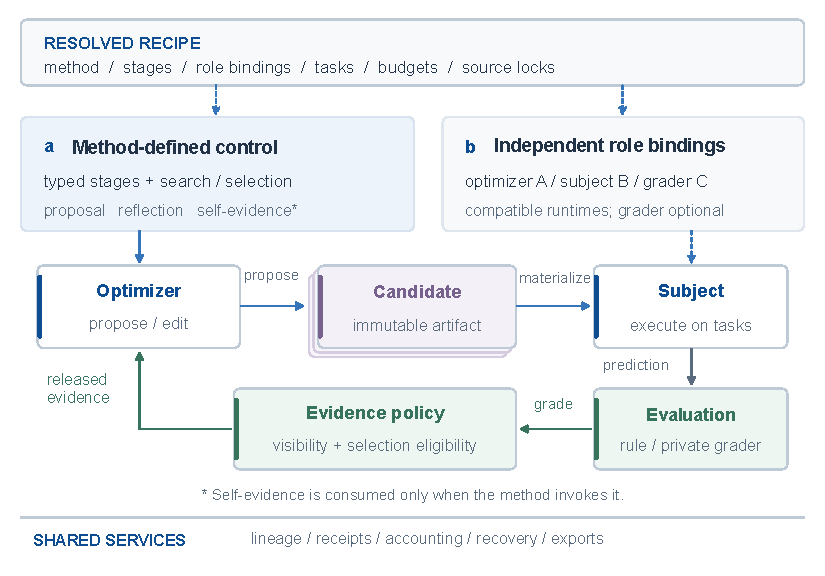
\includegraphics[width=\linewidth]{figures/architecture.pdf}
\caption{\textbf{A common experimental substrate, with method-specific control.} A resolved recipe binds method-defined control and independent harness roles. The central path separates proposal, immutable candidate materialization, and task execution. Formal evaluation returns evidence only through the declared visibility and selection policy. Typed stages, including optional self-evidence, are invoked by the method; the depicted services do not prescribe one universal optimization loop. The lower band preserves common execution records.}
\label{fig:architecture}
\end{figure}

% Role: challenge. Message: the experimental unit includes roles and evidence.
A reproducible self-improvement experiment is larger than an optimizer function. The researcher must identify the exact candidate that ran, the harness and model that proposed it, the subject that executed it, and the evaluator that assigned its score. An interrupted call may have incurred cost without returning a usable result. A hidden test may be recorded for the owner but must remain unavailable to the next proposal. A source edit may exist on disk without ever becoming the executing agent. If these distinctions are implicit, an apparent improvement can instead reflect a changed runtime, leaked feedback, a different selection rule, or missing work.

% Role: method. Message: Proteus separates algorithm from execution contracts.
\proteus{} makes these experimental choices separate, versioned contracts. A \emph{method} owns the optimization loop; \emph{stages} implement typed transformations; \emph{candidates} identify immutable artifacts; and \emph{harness roles} bind model-backed work to execution adapters. Subjects run candidates on tasks, while evaluators produce formal measurements and control their disclosure. Search policies, parallel workflows, persistent workers, accounting, and recovery are shared services rather than mandatory steps in one universal algorithm. Figure~\ref{fig:architecture} summarizes the boundaries.

% Role: advantage. Message: harness agnosticism is bounded role independence.
Harness agnosticism means that a method does not select an adapter through a hard-coded method--harness pair. A recipe can bind a coding proposer and a task subject to the same integration or to different compatible integrations, and can choose their models separately. This is an interface property with concrete limits: a playbook, a prompt overlay, and a source tree still need the correct subject protocol. A supported adapter name does not make every method, role, session mode, or artifact combination valid. Preflight checks and an explicit evidence matrix define the supported subset.

% Role: contribution. Message: the contribution is reusable infrastructure.
The report makes three contributions. First, it specifies a common decomposition of method, typed stage, artifact, harness role, and evaluator, with concrete ACE--Combee and GEPA--Combee compositions. Second, it presents Native as a reference self-evolution method: goals and external scores remain separate, the harness can revise its own tests, and the common profile advances viable candidates without an outer score filter while preserving completed but nonviable candidate edits for repair. Third, it presents a traceable inventory separating historical adapted studies, bounded live role pilots, and source-bound engineering qualification. Existing evolution toolkits already provide extensible infrastructure; the contribution here is the implemented framework and specified Native protocol, not priority for a unified RSI system or a proven quality advantage. Figure~\ref{fig:native} details the Native state transition.

% Role: evidence and boundary. Message: evidence supports an experimental toolkit.
The evidence supports a research toolkit whose available recipes and failure boundaries can be inspected. Historical AIME and Formula runs contain complete declared task splits, while later pilots exercise specific Pi, DSH, and Codex roles. Current preparation checks cover installed extensions, common-trace composition, candidate activation, and a directed CORAL recovery protocol. Their sources and experimental meanings differ, so we do not pool them into a single benchmark or release gate. Generic builders continue to require new model-result qualification. The intended use is to run, inspect, and extend explicitly specified experiments, with missing evidence remaining visible.

\section{Scope and Related Work}
\label{sec:scope}

% Role: definition. Message: fixed-weight improvement does not imply RSI gains.
\paragraph{Experimental scope.}
We study changes to prompts, playbooks, memory, skills, tools, and harness code at fixed model weights. A \emph{harness} is the execution system surrounding a model, including its tools, context handling, and process or session behavior. A \emph{candidate artifact} is the mutable object under study; it need not be the optimizer's harness. We use \emph{self-improvement} for methods that produce and evaluate such changes, without presuming that every trajectory improves. Recursive self-improvement is a research direction that the framework can help investigate. Sustained recursive returns, autonomous expansion of capability, and model training are not demonstrated in this report.

% Role: positioning. Message: prior algorithms retain their separate semantics.
\paragraph{Prompt, context, and program adaptation.}
The five integrated families provide complementary mechanisms rather than interchangeable implementations of one algorithm. GEPA's reflective search and ACE's incremental playbook updates motivate separate search and structured-artifact interfaces. Combee adds an aggregation mechanism usable with more than one base learner. Meta-Harness motivates code artifacts and history-rich proposal workspaces, whereas CORAL motivates independent workers, shared knowledge, and event-triggered interventions. We reuse their published ideas and pinned official implementations where specified, cite their original papers at introduction, and record official software and source revisions in Appendix~\ref{app:pins}. A Proteus integration profile may cover only a subset of an upstream method's options.

% Role: positioning. Message: common evolution infrastructure is established prior work.
\paragraph{Evolution toolkits.}
OpenEvolve provides program-evolution infrastructure~\citep{openevolve_software}, while Penguin Harness supplies multiple RSI toolkits over versioned agent state and shared evaluation records~\citep{penguin_software}. Candidate search, archives, and extensible improvement workflows are established building blocks. Table~\ref{tab:systems} records a bounded source audit of infrastructure and selected method coverage. Proteus's design is described directly in Section~\ref{sec:framework}; the table does not establish overall breadth or performance superiority.

\begin{table}[t]
\centering
\caption{Source-audited system coverage as of November 2, 2026. \yes{}: explicit implementation or documented protocol; \no{}: the named method is not shipped in the inspected built-in registry/library; \unconfirmed{}: the specified shared contract was not established by this audit. A cross does not mean inexpressibility, and a check does not mean matched-paper reproduction. The lower block covers the five method families studied here, not the full method catalog of each system. See Appendix~\ref{app:systems} for scope and pinned sources.}
\label{tab:systems}
\small
\setlength{\tabcolsep}{4pt}
\begin{tabularx}{\linewidth}{@{}Ycc@{}}
\toprule
Interface or integration & Proteus & Penguin \\
\midrule
\multicolumn{3}{@{}l}{\textit{Shared infrastructure and explicit contracts}} \\
Multiple improvement methods & \yes & \yes \\
Versioned candidate resources & \yes & \yes \\
Independent proposer / task models & \yes & \yes \\
Private evaluation / held-out protocol & \yes & \yes \\
Harbor / Docker execution path & \yes & \yes \\
Typed reusable stage / workflow service & \yes & \unconfirmed \\
Separate visibility / selection-eligibility fields & \yes & \unconfirmed \\
Durable dispatch reservation / reconciliation & \yes & \unconfirmed \\
\midrule
\multicolumn{3}{@{}l}{\textit{Built-in adaptations of this report's method families}} \\
GEPA & \yes & \no \\
ACE & \yes & \yes \\
Meta-Harness & \yes & \no \\
Combee & \yes & \no \\
CORAL & \yes & \no \\
\bottomrule
\end{tabularx}
\end{table}




% Role: distinction. Message: Native contributes a method inside the shared toolkit.
\paragraph{A Native method within an extensible framework.}
Proteus pairs the research toolkit with a reference self-evolution method: the executing harness inspects and changes its own declared state, while the protocol keeps the goal, external measurements, and activation rule separate. Its common-contract profile uses viability-gated continuation rather than an outer best-score filter. Pi, DSH, and Codex supply execution integrations rather than competing optimization methods~\citep{zechner_pi_0851,dsh_software,codex_software}. Section~\ref{sec:native} specifies the update rule and the distinction between its legacy and common profiles.

% Role: positioning. Message: reuse execution infrastructure instead of conflating it.
\paragraph{Research toolkits and execution backends.}
The organizational model resembles recipe-oriented research toolkits such as ESPnet~\citep{espnet_software}: expose established methods, common interfaces, and reproducible configurations, while allowing new components to enter at defined extension points. The analogy concerns organization, not comparable maturity or task coverage. Harbor supplies agent evaluation and container infrastructure~\citep{harbor_software}; Proteus uses pinned Harbor/Docker execution where declared, while retaining ownership of method state, candidate identity, feedback policy, and experiment aggregation. Container execution and optimization logic remain distinct responsibilities.

\section{Framework Design}
\label{sec:framework}

% Role: overview. Message: the recipe fixes independent experimental choices.
A resolved recipe specifies the experimental contract before execution. Write this abstractly as
\begin{equation}
\mathcal{R}=(M,\mathcal{S},\mathcal{A},\mathcal{H},\mathcal{T},\mathcal{E},\mathcal{V},\mathcal{B},\mathcal{L}),
\end{equation}
where $M$ is the method, $\mathcal{S}$ its configured stages, $\mathcal{A}$ the artifact protocol, $\mathcal{H}$ role bindings, $\mathcal{T}$ tasks and splits, $\mathcal{E}$ evaluators, $\mathcal{V}$ evidence policy, $\mathcal{B}$ supported budgets, and $\mathcal{L}$ source and dependency locks. This notation summarizes the implementation's separate specifications; it is not a new optimization objective. Locks and an immutable run manifest make changed experimental conditions distinguishable from continuation of an existing run.

\subsection{Methods, stages, and search policies}
% Role: motivation and design. Message: algorithms own control flow.
Method plugins own proposal scheduling, acceptance, stopping, final selection, and private algorithm state. They call framework services through \code{Method.run(services, restored\_state)} and checkpoint the state needed to continue their own loop. Consequently, an ACE sample update does not have to become a Native episode, and a CORAL worker does not have to become a synchronous parent-mutation step. The shared service boundary makes operations comparable at the record level without forcing unlike algorithms into an artificial common schedule.

% Role: design and advantage. Message: stages compose where a method invokes them.
Stages provide typed inputs and outputs for reusable work such as reflection, code proposal, or self-assessment. A stage obtains model-backed behavior through its configured actor rather than creating an unrecorded provider call. Sequential, conditional, finite-loop, map, and workflow composition support the implemented profiles. Adding a stage declaration alone does not insert it into every method: the method must expose or invoke that stage and specify how its output affects later actions. A new update rule or control loop therefore requires a plugin when no existing configurable mechanism expresses it.

% Role: definition. Message: candidate search and archive sampling are policies.
Search services separate the generation of candidates from decisions about their retention and reuse. An archive is an inspectable set of candidate records and eligible measurements. Parent selection chooses which archived candidates condition a proposal; archive policy decides what to retain; final selection determines the output candidate. These decisions receive a permitted score view and a supplied random-number generator, and return candidate identifiers with reasons. Scalar, uniform, and Pareto-style policies are useful components, but are not aliases for a full upstream algorithm. The GEPA profile additionally retains its pinned instance-frontier and parent-sampling semantics.

\subsection{Candidate identity and harness roles}
% Role: motivation and design. Message: candidate identity persists across actors.
Candidates are immutable, content-addressed artifacts with explicit parent edges. The artifact store supports text components, structured records, and file trees, together with checked deltas and materialization. A candidate identifier refers to the object that was proposed; its lineage records the update's origin. Running that candidate additionally requires an execution configuration. The system therefore records both artifact identity and effective runtime identity, including a pinned base and projection when a prompt component is overlaid on a source tree. Deleting a declared component removes the corresponding base path instead of silently restoring old content.

% Role: design. Message: one harness integration supplies independently configured roles.
A \code{HarnessIntegration} binds an adapter factory, source identity, options, and declared capabilities to versioned role plugins. Ordinary actors, coding workspaces, and Native evolution roles use the roles that the integration advertises. Each recipe independently supplies an \code{ActorSpec}, including model and runtime options, for the optimizer or proposer, subject, and optional grader. The factory can know the role without knowing the optimization method. This supports both same-harness experiments and compatible cross-harness bindings without maintaining a separate registry for every method--harness pair.

% Role: boundary. Message: capability and artifact checks limit interchangeability.
Role independence does not erase representation or lifecycle requirements. The common candidate subject runs a file tree, or an explicitly declared projection, through its configured actor and reads the task prediction from the specified output path. A GEPA text-component candidate and an ACE playbook require their own compatible projections or runners. Source validators check the exact candidate before execution; missing output, invalid source, and infrastructure failure remain distinct outcomes. The common candidate bridge currently requires independent serial target trials, and its materialization layer is trusted host execution rather than a process sandbox. Container adapters supply only their declared additional boundary.

\subsection{External evaluation and evidence visibility}
% Role: motivation and design. Message: evaluation is separate from proposal work.
Evaluation consumes a task, a recorded subject prediction, and any private reference through a declared evaluator. Deterministic exact-match or domain-specific graders share this interface with a managed model-judge protocol. In the latter, a separate grading actor receives private input and produces an identity-bound result with its own usage record. The implemented managed grading context permits one dispatch; a multi-call judge needs an explicitly bounded protocol. A malformed grading response is an infrastructure failure with an unavailable score, not a negative task outcome fabricated to complete a table.

% Role: design and advantage. Message: availability and eligibility are different.
Feedback visibility and selection eligibility are independent experimental choices. A visible score can inform learning where the method permits it; a hidden reference, grader request, or final score remains outside optimizer inputs. A measurement can also be recorded without being eligible for parent or final selection. Owner-side private export is separate from what an agent sees. These boundaries allow several evaluators to coexist and permit validation selection followed by hidden testing without treating all recorded numbers as optimization feedback. They govern supplied evidence; trusted Python plugins still require appropriate execution isolation if adversarial behavior is in scope.

% Role: boundary. Message: self-evidence is not an external quality score.
A self-evaluation stage produces evidence whose author and consumption rule must be explicit. It can inspect allowed traces, critique a candidate, or propose additional checks, provided the chosen method invokes it. Its output does not automatically replace the independent external score or become a hidden-test oracle. The framework can preserve both channels, enabling later experiments on whether self-evidence is useful, calibrated, or misleading. Current extension examples demonstrate this separation mechanically; they do not establish the quality of self-authored evaluators.

\subsection{Execution, accounting, and recovery}
% Role: design. Message: environment lifecycle is explicitly declared.
Execution services distinguish a trial, an explicit sequence with carried state, and a persistent worker lifecycle. Pinned Harbor/Docker profiles can provide candidate loading, independent verification, source builds, and cleanup evidence. A persistent worker additionally needs a durable identity, its own workspace, a session policy, and a way to submit immutable candidates for formal evaluation. Shared knowledge uses versioned, sourced records and compare-and-swap publication; event policies can request reflection, consolidation, or a change of direction. The existence of a shared snapshot is not proof that another worker consumed it.

% Role: design and boundary. Message: accounting preserves uncertainty.
The managed ledger reserves resources before dispatch and settles observed usage against the corresponding operation. Optimizer, subject, grader, build, retry, and worker activity retain attributable records within their supported boundaries. A reservation is not an invoice. Unknown tokens, provider-call counts, monetary charges, or elapsed intervals remain unknown; unsupported finite limits fail preflight. A terminal operation with incomplete usage differs from an operation whose external completion is unknown. In the latter case, the unresolved reservation and dispatch state prevent an ordinary resume from silently issuing the work again.

% Role: design and advantage. Message: recovery reuses facts rather than reconstructing success.
Recovery restores method checkpoints and committed operation results under the original source and configuration locks. Backend-specific receipts can reconcile independently completed work, including the supported Harbor worker path. Without trustworthy completion evidence, the system stops for reconciliation instead of inferring that a timeout means no work occurred. Candidate failure also remains inspectable: A completed Native staged-source episode preserves a nonviable candidate for repair while subsequent execution retains the last valid source. Its activation proof binds the next executing source or binary to the validated artifact. These guarantees concern supported state transitions and receipts, not universal recovery from every provider or worker failure.

\subsection{Inspection and researcher interfaces}
% Role: design. Message: the viewer and generic exports have different scopes.
Inspection has two complementary surfaces. The local Native viewer exposes Evolution, Measurements, Configuration, and Snapshots for sweep records. It distinguishes failed candidates from active checkpoints and preserves missing metrics. Generic recipes instead export JSON and CSV records for tasks, candidates, lineage, operations, usage, and timing; study specifications aggregate explicitly declared conditions and seeds. The Native viewer does not currently render every generic recipe. Descriptive surface or trajectory distances are available for supported artifacts, but are not universal quality measures across prompts, memory, and source code.

% Role: design and advantage. Message: external extensions use a finite public API.
The versioned \code{proteus.api.v1} surface exposes contracts and services for methods, stages, subjects, evaluators, actors, artifacts, and search policies. Release preparation freezes 100 public exports and 64 contract schema identities. External templates cover method, stage, evaluator, subject, and policy extensions and have installed-distribution checks outside the checkout. Private SQL tables, journal layout, and arbitrary internal service fields are not made stable merely by importing a public type. A new contribution must declare its capabilities, source identity, feedback use, and recovery behavior alongside its algorithm.

\section{Native Self-Evolution and Composable Recipes}
\label{sec:recipes}

\subsection{Native: goal-aware, viability-gated self-evolution}
\label{sec:native}

% Role: motivation. Message: a supplied measurement need not exhaust the objective.
Native studies self-evolution when the objective is not necessarily identical to an external score. A natural-language goal can be fully operationalized by a benchmark, or only partly measured by it. The default protocol asks the harness to judge that relationship and to add or revise its own tests when useful. It does not mandate extra tests or treat a self-reported score as an independent measurement. The legacy interface also permits a goal without an evaluator, or open-ended exploration without a supplied goal; those are explicit settings rather than evidence of autonomous capability growth.

% Role: method. Message: the running harness proposes changes to its own declared state.
The reference episode uses \emph{observe, propose, act, reflect}. The active harness inspects its state and permitted evidence, chooses a scoped change, edits its pending candidate, and records outcomes and unresolved risks. The four phase names alone are not the contribution. The relevant experimental choices are which goal and evidence are supplied, what state the harness can change, which implementation executes each phase, and how a candidate becomes active. For supported staged-source adapters, all phases run the frozen last-valid source, including reflection; pending edits take effect only after validation and activation. Self-authored tests remain part of the harness state, distinct from the external grader.

% Role: formalization. Message: the common profile has an explicit non-score admission rule.
The common-contract profile separates the active harness $A_t$ from the working candidate $W_t$. For an episode that completes successfully and publishes a candidate, let it produce $\widetilde W_{t+1}=F_\theta(A_t,W_t,G,V_t)$, where $G$ is the supplied goal, $V_t$ is permitted evidence, and the model weights $\theta$ remain fixed. With a model-free viability check $v$, its transition is
\begin{equation}
 W_{t+1}=\widetilde W_{t+1},\qquad
 A_{t+1}=\begin{cases}
 \widetilde W_{t+1}, & v(\widetilde W_{t+1})=1,\\
 A_t, & v(\widetilde W_{t+1})=0.
 \end{cases}
\label{eq:native-transition}
\end{equation}
There is no condition requiring an external score to increase. A viable candidate becomes active even if its measured task score decreases; an invalid candidate remains the exact working state for a later repair episode while execution retains $A_t$. An actor/stage failure or an uncertain external operation stops this transition and follows the shared failure/recovery protocol; it is not silently treated as a viability rejection. This defines a continuation policy, not a monotonic-improvement guarantee. The final candidate is the last valid one, not an outer-loop score maximum.

\begin{figure}[t]
\centering
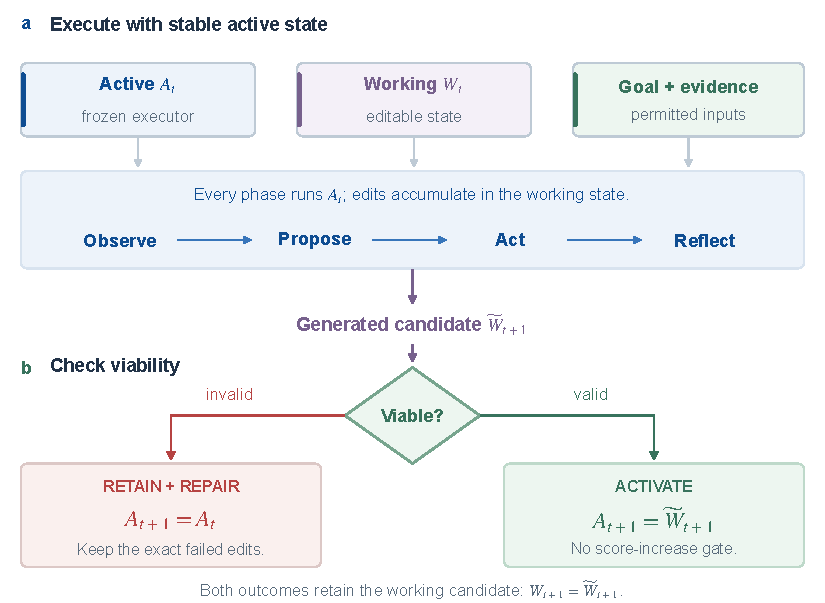
\includegraphics[width=\linewidth]{figures/native-transition.pdf}
\caption{\textbf{Native common-profile transition.} The current active harness executes the episode while changes accumulate in a separate working candidate. A source-bound viability result controls activation. Completed but nonviable edits remain available for repair, and formal scores enter later reasoning only through the declared evidence policy; they do not implement an outer acceptance filter. This figure describes supported staged-source execution, not every legacy adapter's lifecycle.}
\label{fig:native}
\end{figure}

% Role: scope. Message: the two Native profiles must not be conflated.
The common profile requires observed evaluation pools, evaluates the initial and each viable candidate, and runs optional hidden tests after evolution. It binds evolution and subject roles to the same harness integration and uses exactly one managed episode stage. Its supported phase controls do not make it an arbitrary stage graph. Legacy Native retains its separate goal/no-goal options, evaluator schedules, dispositions, measurements, and selection settings. Accordingly, the no-outer-score rule in Equation~\ref{eq:native-transition} describes the common profile; it must not be generalized to every legacy configuration.

% Role: evidence and limitation. Message: current evidence supports the mechanism, not its advantage.
The source-bound Native fixture demonstrates invalid-edit retention, later repair, changed candidate execution, private final grading, and replay. Bounded Pi/DSH pilots additionally exercise one common episode; the broader engineering record tests supported source activation paths. These support the implemented state transition. They do not establish that goal-aware self-evolution beats score-guided search, that self-authored tests are useful, or that useful improvements compound. Such claims require matched comparisons varying objective framing, evidence access, activation/selection policy, and self-evidence while holding tasks, models, initial artifacts, and budgets fixed.


\subsection{Reference recipes and researcher workflow}

% Role: overview. Message: recipe reuse preserves method semantics.
The included recipes demonstrate several ways to reuse infrastructure without equating their algorithms. Table~\ref{tab:profiles} identifies the optimized artifact, controlling mechanism, and empirical boundary of each family. The method documentation and frozen profile configurations specify the actual options; family names alone are insufficient to reconstruct an experiment. In particular, an original-domain builder is an entry point for preparing a new study, not a certificate that the resulting configuration has model-quality evidence.

\begin{table}[t]
\caption{Implemented profile boundaries. Reuse is explicit at the artifact, stage, or service layer. A family name is not a claim of all upstream options or matched-paper results.}
\label{tab:profiles}
\small
\begin{tabularx}{\linewidth}{@{}>{\raggedright\arraybackslash}p{0.14\linewidth}>{\raggedright\arraybackslash}p{0.17\linewidth}Y Y@{}}
\toprule
Family & Candidate & Included mechanism & Evidence boundary \\
\midrule
GEPA & Text components & Single-mutation loop, instance frontier, round-robin components & Adapted AIME study; no merge/cache in this profile. \\
ACE & Structured playbook & Generator, reflector, curator; incremental updates; offline/online & Adapted Formula studies; online stream differs from final held-out scoring. \\
Meta-Harness & Memory-system code & Historical evidence retrieval, proposal workspace, learning and selection & Historical JSON proposer; actual coding proposers have bounded pilots. \\
Combee & Base-method artifact & ACE/GEPA aggregation, parallel maps and fixed/dynamic batches & Formula results and separate model-free common trace; no isolated speedup. \\
CORAL & Program and shared knowledge & Worker generations, formal submissions, sourced knowledge, event policies & Adapted circle packing; separate three-request directed qualification. \\
Native & Harness source/state & Legacy compatibility; additional common-stage evolution profile & Source activation/repair and external evaluation; no universal Native phase requirement. \\
\bottomrule
\end{tabularx}
\end{table}


% Role: example. Message: ACE and Combee compose at a real reusable boundary.
\paragraph{ACE with Combee.}
ACE's generator, reflector, and curator operate on a versioned playbook whose structured updates retain stable entries and counters. Combee-ACE reuses that representation and the surrounding evaluation services, while introducing grouped parallel proposal work and aggregation before publication. The implementation distinguishes original samples from copied aggregation occurrences and preserves their provenance. Sequential ACE, naive parallel, fixed Combee, and dynamic Combee therefore form explicit conditions rather than informal choices of thread count. The common frozen-trace check in Section~\ref{sec:mechanism} isolates these consumption and update mechanisms.

% Role: example. Message: GEPA and Combee compose without replacing the search loop.
\paragraph{GEPA with Combee.}
Combee aggregation is also integrated into the pinned GEPA search loop. GEPA retains candidate evaluation, acceptance, component choice, and final testing, while the aggregation operator changes how reflective proposals are formed. This is a second implemented composition, with its own artifact and parser requirements. The existence of both integrations supports component reuse across base learners; it does not establish that a Combee operator can be attached to any method without adapting its input and update contracts. The historical Formula results in this report concern Combee-ACE, not a new Combee-GEPA benchmark.

% Role: example. Message: a self-evaluator is an explicit experiment intervention.
\paragraph{An explicit self-evaluation experiment.}
A stage-composing method can insert a self-evaluator between a proposal and the next method decision. The researcher declares its inputs, the permitted evidence view, the output type, and whether that output affects revision, selection, or only logging. An ablation can then remove or replace the stage while keeping tasks, external grading, budgets, and other choices fixed. The tutorial demonstrates such configuration and plugin boundaries. It supplies a way to pose the research question; a useful or calibrated self-evaluator would still require independent empirical validation.

% Role: example and boundary. Message: Native is one implementation, with two paths.
\paragraph{Native evolution as a method.}
The legacy Native compatibility recipe preserves the existing episode transaction engine and its evaluator schedules and measurements. The additional common Native evolution profile uses ordinary stages, immutable candidates, shared evaluation, and the recovery journal while retaining observe/propose/act/reflect inside its episode stage. It uses neutral disposition and last-valid activation, not outer-score selection. The same integration supplies its evolution and target roles. These paths are documented separately; neither is imposed on ACE, GEPA, Meta-Harness, Combee, or CORAL.

% Role: workflow. Message: configure existing behavior, extend missing behavior.
\paragraph{From an experiment idea to a run.}
The normal workflow is to choose a profile, bind compatible actors and artifacts, declare tasks and evidence policy, then validate and lock sources before running. Replacing an implemented model, prompt, policy, budget, or exposed stage is a configuration change. Introducing a new update rule, actor protocol, or side effect requires the corresponding plugin and its checks. Resume uses the original locks; a changed method or runtime creates a new experiment. Thus, ``no model training'' is not sufficient for configuration-only reproduction of an arbitrary new method.

% Role: ecosystem. Message: skills provide guidance rather than performance.
\paragraph{Agent-facing use and contribution skills.}
The accompanying documentation commit includes a \code{proteus-use} skill that guides an agent through profile choice, role binding, validation, execution or saved-run analysis, recovery, and reporting. An optional \code{proteus-contribute} skill guides extension work. These repository-distributed instructions reference the matching runtime and documentation, distinguish an analysis-only request from a new experiment, and keep evidence and resource limits explicit. They are a usability and contribution interface, not an additional optimizer or a demonstrated performance contribution. Their committed documentation provenance is recorded separately from the source revisions that produced the experimental evidence.

\section{Evidence and Supported Conclusions}
\label{sec:evidence}

% Role: setup. Message: separate the three evidence strata.
We evaluate the framework through three distinct evidence strata: historical adapted model studies, bounded live harness-role pilots, and source-bound engineering qualification. The historical inventory contains fourteen adapted method profiles and one Native mechanism profile across sixteen recipes; one profile can contain more than one recipe. These are archived experiments from earlier source revisions, not reruns of the current release-preparation tree. The pilot matrix tests specified role bindings on small tasks. Engineering checks test execution contracts and recovery rather than model quality. Appendix~\ref{app:evidence} links each stratum to its source and records what was inspected for this report.

% Role: setup and boundary. Message: retain original model and budget semantics.
Historical AIME and Formula configurations use the recorded \code{deepseek-flash} model identifier with temperature zero and thinking disabled. AIME uses an 8,192-token response limit; the Formula roles use 4,096. These are the identifiers and settings in the archived configurations, not assertions of equivalence to an upstream paper's model or to an unreported provider-resolved revision. Model seeds do not establish deterministic remote inference. We retain baseline, selected, and last-candidate distinctions, report task counts directly, and avoid pooled cross-task rankings or single-seed significance claims.

\subsection{Historical task results: examples of supported study protocols}
\label{sec:historical}
% Role: evidence. Message: different evaluation protocols require different labels.
The AIME and standalone Formula studies illustrate why a shared record format must retain evaluation semantics. GEPA/AIME uses 45 training, 45 validation, and 30 private tasks; its recorded baseline solves 23 private tasks and its selected candidate solves 24. ACE/Formula uses 500/300/200 tasks. Offline ACE records 141/200 for the initial playbook and 173/200 for the selected playbook, while online ACE records 163/200 pre-learning stream predictions against a 141/200 baseline. The online number describes predictions made before each learning window, not an untouched test of the final playbook. Table~\ref{tab:historical} keeps these quantities separate.

\begin{table}[t]
\caption{Historical adapted single-seed results. Counts are correct tasks / evaluated tasks. Offline selected-candidate results and online stream predictions have different meanings; these rows are not a cross-task ranking.}
\label{tab:historical}
\small
\centering
\begin{tabular}{@{}lrrl@{}}
\toprule
Profile & Initial & Reported outcome & Evaluation meaning \\
\midrule
GEPA / AIME & 23/30 & 24/30 & Selected, private \\
ACE / Formula offline & 141/200 & 173/200 & Selected, private \\
ACE / Formula online & 141/200 & 163/200 & Pre-learning stream \\
\bottomrule
\end{tabular}
\end{table}


% Role: interpretation. Message: selection provenance matters even with complete results.
Offline ACE also shows why selecting the last artifact would change the reported experiment. The retained candidate is selected after 200 training examples, whereas the last playbook follows all 500. Only the initial and selected playbooks have private measurements; the last playbook's private score is unavailable. Proteus records the selected candidate, the final execution artifact, their hashes, and the visible-only selection rule separately. The 16-percentage-point observed difference is a result of this one adapted trajectory, not a claim about expected gain or the last candidate.

% Role: evidence. Message: code artifacts enable a distinct adapted protocol.
The historical Meta-Harness-inspired study covers USPTO, Symptom2Disease, and LawBench with NoMemory and FewShotAll baselines plus three generated memory programs. Its proposer makes one JSON call that returns three programs, rather than conducting the original paper's extended tool-using coding search. Each system has 450 learning callbacks and 260 visible predictions over 130 distinct visible tasks. Four selected systems receive 412 private tasks each. Table~\ref{tab:mce} reports their per-domain counts; the generated systems do not dominate FewShotAll. This experiment demonstrates a code-artifact and learning/evaluation protocol under its recorded adaptation, while current coding-proposer support is assessed separately by pilots.

\begin{table}[t]
\caption{Historical Meta-Harness-inspired MCE private results. The proposer is one JSON call producing three programs; four systems were selected for private evaluation. The unselected lesson-distilled program has no private result. Counts are correct / tasks, and generated systems do not dominate FewShotAll.}
\label{tab:mce}
\small
\centering
\begin{tabular}{@{}llrrr@{}}
\toprule
System & Origin & USPTO & Symptom2Disease & LawBench \\
\midrule
NoMemory & Baseline & 16/100 & 151/212 & 28/100 \\
FewShotAll & Baseline & 29/100 & 183/212 & 55/100 \\
Contrastive boundary & Generated & 29/100 & 162/212 & 45/100 \\
Dual-pool retrieval & Generated & 30/100 & 152/212 & 52/100 \\
\bottomrule
\end{tabular}
\end{table}


% Role: evidence and limitation. Message: multiworker completion is not cooperation benefit.
The historical CORAL-inspired circle-packing arms compare one proposer making 20 submissions with two proposers making ten each, using one evaluation worker. The recorded selected normalized scores are 0.928722 and 0.900208, respectively, from an initial 0.364102. Twelve versus eleven submissions succeed; eight versus nine time out. Final confirmation repeats the same public 26-circle problem. These results do not establish a multiworker advantage, hidden-task generalization, or the behavior of the original persistent native agents. The locally unrecovered historical cross-worker chains are not repaired by relabeling a later protocol check.

\subsection{Composition: historical measurements and a controlled trace}
\label{sec:mechanism}
% Role: evidence. Message: costs and timings have their own observable boundaries.
The Combee/Formula inventory contains sequential ACE, naive parallel, fixed Combee, and dynamic Combee in both offline and online modes. The four online conditions have accepted pre-learning accuracy, independently recorded API upper-cost estimates, and study elapsed measurements (Table~\ref{tab:combee}). The API amounts are not invoices and do not overwrite unknown canonical native USD totals. Study elapsed time includes the recorded study boundary and differs from the sum of overlapping operation durations. Shared host resources and continuation histories prevent interpreting the table as an isolated speedup experiment; the different baseline scores also remain visible.

\begin{table}[t]
\caption{Historical online Combee/Formula conditions, seed 0. Accuracy is pre-learning stream correct / 200. API upper cost is USD, not an invoice or canonical native cost. Elapsed hours follow the recorded study timer; shared resources and continuations preclude an isolated speedup claim.}
\label{tab:combee}
\small
\centering
\begin{tabular}{@{}lrrrr@{}}
\toprule
Condition & Initial & Stream & API upper (USD) & Study elapsed (h) \\
\midrule
ACE & 139/200 & 160/200 & 1.738 & 4.62 \\
Naive & 137/200 & 157/200 & 0.705 & 2.81 \\
Fixed & 140/200 & 159/200 & 0.772 & 3.00 \\
Dynamic & 137/200 & 162/200 & 0.742 & 2.89 \\
\bottomrule
\end{tabular}
\end{table}


% Role: evidence. Message: fixed inputs isolate composition mechanics.
A separate model-free check feeds eleven frozen original task/prediction/feedback/reflection records to the four production ACE variants. All arms use the same H0 and seed. Sequential ACE curates each example; naive parallel uses batches 3/3/3/2; fixed Combee uses the same batch schedule with copied groups and reduction; dynamic Combee uses 1/2/4/4 under a controlled clock. Curator invocation counts are 11, 4, 12, and 12, respectively, while every arm makes 22 generator invocations. Provider-call count is zero. The auditor binds actual payload bytes, source/configuration locks, grouping, requests, updates, and lineage. This establishes distinct, reusable composition semantics under common inputs; synthetic timing and deterministic responses cannot establish learned quality or model speedup.

\subsection{Harness-role interoperability: sixteen bounded live cells}
\label{sec:pilots}
% Role: evidence. Message: explicit cells support role-level portability.
The live pilot inventory contains sixteen accepted cells across Pi, DSH, and Codex (Table~\ref{tab:pilots}). Native and GEPA cells use actual Pi/DSH source adapters as task subjects; GEPA's reflector is a separately managed chat actor. Other cells put the coding harness in the ACE/Combee generator role, Meta-Harness proposer role, or a bounded CORAL worker wrapper. The tasks are deliberately small and their role placement is part of the evidence. A checkmark therefore means that the named minimum cycle was observed, not that all roles of a complete benchmark ran on that harness.

\begin{table}[t]
\caption{Sixteen accepted bounded live cells. \yes{} = the listed minimum cycle has source-bound live evidence; \na{} = not established by this pilot inventory. The harness role differs by row. These are integration pilots, not full benchmarks or comparisons of model quality.}
\label{tab:pilots}
\small
\begin{tabularx}{\linewidth}{@{}p{0.18\linewidth}cccY@{}}
\toprule
Method/profile & Pi & DSH & Codex & Role exercised by the named harness \\
\midrule
Native common & \yes & \yes & \na & Evolution actor and candidate subject; one episode. \\
GEPA & \yes & \yes & \na & Candidate subject; separate managed chat reflection. \\
ACE & \yes & \yes & \yes & Generator executing the current playbook. \\
Combee-ACE & \yes & \yes & \yes & Independent generator workspaces; one map/reduce batch. \\
Meta-Harness & \yes & \yes & \yes & Coding proposer; generated memory-system programs execute. \\
CORAL bounded & \yes & \yes & \yes & One supervised worker; two fresh coding workspaces. \\
Combee-GEPA & \na & \na & \na & Implemented composition, outside this live matrix. \\
\bottomrule
\end{tabularx}
\end{table}


% Role: interpretation. Message: successful integration can include no quality gain.
Successful cycles include outcomes that do not improve on their baselines. The Pi ACE and Combee-ACE pilots modify and execute a playbook but retain the initial candidate, with private scores unchanged at zero. Meta-Harness coding proposers generate executable systems, yet the selected baselines tie or exceed them on the observed pilot tasks; those generated systems need not have private scores. Other cells demonstrate a changed policy or source artifact, independent scoring, and zero additional dispatches on completed resume. These outcomes support interoperability and auditability while resisting an artificial all-positive performance story.

% Role: boundary. Message: live cells do not prove universal compatibility.
The matrix leaves Codex Native/GEPA and all Combee-GEPA live role cells unclaimed. The additional CORAL role pilots use one supervised worker invoking fresh coding workspaces, not persistent native-session multiworker execution. Requested/applied model identifiers are preserved separately from missing provider-resolved identities. Cell-level evidence spans several recorded commits and includes corrected failed attempts. It is appropriate for the bounded integration claim, but cannot be assembled into a single-source release gate or a controlled comparison of harness quality.

\subsection{Current engineering and directed protocol qualification}
% Role: evidence. Message: direct delivery is stronger than availability alone.
A directed CORAL qualification specifically tests shared-content delivery, intervention, and controller-crash recovery. The accepted live run contains exactly three completed paid provider requests, reporting 1,141 input tokens and 113 output tokens; USD cost is unknown. Readback follows the actual delivered content, applied intervention, original request identities, and settled receipts. Resume performs the declared final confirmation evaluation without an additional model request. This closes a narrow protocol chain that historical knowledge snapshots alone could not prove. It does not establish worker-crash recovery, native model-session continuation, simultaneous provider dispatch, or a benefit from collaboration.

% Role: evidence. Message: a full preparation smoke is mechanism qualification.
The complete preparation smoke, run \href{https://github.com/proteus-evolve/Proteus/actions/runs/41398194611}{41398194611}, passes Offline, Minimal, LLM, Pi, DSH, and Codex jobs in one source-bound run. The offline job reports 1,842 passing tests and 91 skips; the live jobs include the declared source-edit, activation, and rejection checks. This is engineering qualification. Pi/DSH diagnostic archives are bounded and sanitized: Pi's 20 phase outcomes and 20 of DSH's 24 outcomes return 137 under controller caps, with incomplete usage streams. Codex's original strict-checker log establishes its checked edit/binary behavior, but its raw trace, snapshot, and binary archive were not exported. Passing this bounded gate neither proves complete billing nor makes the retained artifacts a full replay archive.

% Role: evidence. Message: reports can be reconstructed without new inference.
Independent generic readback reconstructs nine report/CSV files for each of five saved runs, covering 92 task rows and 30 candidates with no unreported rollout. Costs and timing intervals that were missing remain missing. Installation evidence covers 22 checks outside the checkout, including extension templates, exports, and study comparison. These results support the usability of the records and public extension boundary. They do not measure researcher productivity, and the current report does not rerun models, containers, or benchmarks to reproduce them.

% Role: interpretation. Message: each evidence stratum answers a different question.
Taken together, the evidence shows implemented algorithm profiles, concrete role-level execution, and inspectable state transitions under declared conditions. Historical task improvements illustrate that the substrate can carry substantive studies; negative pilot outcomes and retained failures show why implementation acceptance is a separate criterion. Controlled trace checks expose reusable mechanics, and directed qualification tests a specific recovery chain. None of these alone establishes a general self-improvement advantage, a universal harness interface, or a successful future release tag.

\section{Limitations and Research Directions}
\label{sec:limits}

% Role: limitation. Message: statistical and causal claims need new evidence.
The principal empirical limitation is the absence of matched, multi-seed comparisons across the implemented methods and harness choices. Historical profiles use adapted models, different algorithm settings, source revisions, and task protocols. The bounded coding-proposer pilots do not replace full coding-search benchmarks. To estimate an effect of a framework component, a study must hold its task splits, models, starting artifacts, feedback, selection, and enforceable budgets fixed while varying that component. The present evidence does not estimate population-level gains, state-of-the-art performance, or the causal contribution of composition, self-evaluation, or shared knowledge.

% Role: limitation. Message: extensibility is not arbitrary support.
Native's viability gate establishes executability, not useful improvement. A runnable regression can become the active candidate, and self-authored tests can be incomplete or misleading. Matched objective-framing, score-selection, and self-evidence ablations are needed before claiming a quality benefit.

% Role: limitation. Message: extensibility is bounded by contracts.
The framework's modularity is limited by implemented artifact and execution contracts. Some new research ideas need a new stage or policy; others require a method, subject, evaluator, runtime, or service extension. Session continuity, concurrency, and isolation are capabilities rather than freely interchangeable options. Plugins executing in the controller are trusted, and the common subject materializer is not itself a sandbox. A richer support matrix requires actual contract and execution evidence for the new combinations, not additional configuration labels. Native compositions with ACE, GEPA, Combee, or CORAL are reserved for a later version; this report covers ACE--Combee and GEPA--Combee.

% Role: limitation. Message: inspectability has observability and archive limits.
Accounting and inspection are constrained by what providers and harnesses expose. Unknown provider-call totals or monetary charges remain unknown, and upper-cost estimates retain their separate meaning. Completed-resume checks cannot establish recovery from every uncertain external effect. The directed CORAL result covers a controller interruption, not a worker or native-session crash. Bounded Pi/DSH diagnostics and the Codex checker-only archive limit independent reconstruction of full native conversations and binaries. Generic JSON/CSV reports and the Native interactive viewer also have different current coverage.

% Role: comparison boundary. Message: architecture differences have not been measured head to head.
The coverage table is a source audit, not a controlled evaluation. Its selected method rows do not establish overall breadth or maturity. Integration-effort studies should measure the changes needed to add a stage or method under fixed task and runtime conditions; interruption studies should test retained evidence and continuation decisions. Until then, configurability, reliability, and research productivity remain implemented mechanisms and research hypotheses rather than measured comparative advantages.

% Role: future research. Message: there are concrete next experiments, not hidden requirements.
The next research steps are matched harness-role ablations, full coding-proposer studies, multi-seed method comparisons, and controlled tests of self-evidence and cross-worker knowledge use. A particularly useful design would compare the same candidate update under different proposer/subject bindings while preserving the evaluator and allowed evidence. Long-horizon experiments are additionally needed before making claims about sustained recursive improvement. These are open research questions; their absence narrows the conclusions of this report rather than invalidating the supported infrastructure claims.

\section{Conclusion}
% Role: conclusion. Message: unified contracts support extensible experiments.
\proteus{} combines a modular experiment framework with the Native self-evolution reference method. The framework separates methods, artifacts, harness roles, and evaluation; Native specifies goal/evidence use, viable-candidate activation, and nonviable-edit repair. Implemented compositions, historical studies, bounded pilots, and engineering checks establish inspectable execution within declared limits, not a general quality advantage. The interface records what changed, what executed, and what remains unknown, enabling controlled investigation of self-improvement methods.

\FloatBarrier
\clearpage
\begingroup
\setlength{\bibsep}{3pt plus 1pt}
\bibliographystyle{iclr2027_conference}
\bibliography{references}
\endgroup
\clearpage
\appendix
\section{Source Pins and Attribution}
\label{app:pins}

Each method is cited by its original paper and official code. The paper version identifies the reference text; the commit identifies the reused implementation. Neither identity establishes that a Proteus experiment matches all original model, budget, split, or runtime choices. Full adaptation notes are in the source-pinned \repo{docs/METHOD_REFERENCES.md}{method reference record}. Table~\ref{tab:pins} lists the software pins used by the integrations.

\begin{table}[H]
\caption{Original papers and official implementation pins. Linked commits contain full revision identities. Combee aggregation and dynamic sampling use different source revisions.}
\label{tab:pins}
\small
\begin{tabularx}{\linewidth}{@{}p{0.15\linewidth}p{0.18\linewidth}Y@{}}
\toprule
Method & Paper version & Official software / pinned code \\
\midrule
GEPA & 2507.19457v2 & \href{https://github.com/gepa-ai/gepa/tree/8b0ce6cd99a234f6b74daf37558a2ac0ce18f975}{gepa-ai/gepa: 8b0ce6cd99} \\
ACE & 2510.04618v3 & \href{https://github.com/ace-agent/ace/tree/82709de050e1db6e6ef2f07bcb0393560b94992a}{ace-agent/ace: 82709de050} \\
Meta-Harness & 2603.28052v1 & \href{https://github.com/stanford-iris-lab/meta-harness/tree/8123ccabe2b19fa1123090b2e5f1bacc20963ce8}{stanford-iris-lab/meta-harness: 8123ccabe2} \\
Combee & 2604.04247v2 & \href{https://github.com/gepa-ai/gepa/tree/f1cfdee2856e9dc4b5b4dc5cc2e391d0aa20d819}{gepa-ai/gepa aggregation: f1cfdee285}; \href{https://github.com/gepa-ai/gepa/tree/f9e2d430815e5a0b36d58d1dab2f36f8082759e4}{dynamic sampler proposal: f9e2d43081}; Formula also uses ACE above. \\
CORAL & 2604.01658v3 & \href{https://github.com/Human-Agent-Society/CORAL/tree/0123dfb939b35228cf2c1fde224cd0561e727408}{Human-Agent-Society/CORAL: 0123dfb939} \\
\bottomrule
\end{tabularx}
\end{table}


The historical Native activation profile uses Pi v0.85.1 at \code{d981de1229}; the later Pi role pilots instead pin \code{914cf1472e}, while the DSH pilots pin \code{99f6f02fec}. These software identities are distinct from the method-code pins above. Codex's individual run records retain its source and binary bindings; a successful strict checker does not imply that its raw binary archive was exported.

\section{Additional Historical Results and Interpretation}
\label{app:fullresults}

Table~\ref{tab:offline} preserves all five historical offline Formula conditions: standalone ACE and the four arms of the Combee study. All test denominators are 200. Separate runs have separate H0 measurements. Parallel arms use eight workers; the fixed batch parameter is 50. The dynamic offline trajectory mostly uses batch size one, and is not evidence of an effective large-batch speedup. The naive condition is the accepted fresh-H0 v7 replacement; earlier failures are retained in the historical archive rather than mixed into its result.

\begin{table}[H]
\caption{Historical offline Formula results, seed 0. Selected-candidate private counts are shown, with an explicit selected-equals-last indicator. Canonical cost and continuous elapsed-time gaps are retained in the archived records; API upper estimates are a separate field.}
\label{tab:offline}
\small
\centering
\begin{tabular}{@{}lrrcr@{}}
\toprule
Condition & Initial & Selected & Selected = last & API upper (USD) \\
\midrule
Standalone ACE & 141/200 & 173/200 & \no & 5.346 \\
Combee study: ACE & 136/200 & 174/200 & \yes & 5.504 \\
Naive parallel (v7) & 139/200 & 168/200 & \yes & 1.498 \\
Fixed Combee & 139/200 & 170/200 & \yes & 1.633 \\
Dynamic Combee & 138/200 & 174/200 & \yes & 2.976 \\
\bottomrule
\end{tabular}
\end{table}


The model-cost field in Tables~\ref{tab:combee} and \ref{tab:offline} is an accepted physical-API upper estimate, not a canonical native ledger total or invoice. Offline continuous elapsed time is unavailable. Summing controller intervals across continuations does not recover an uninterrupted duration or process downtime. Historical MCE likewise preserves unknown canonical cost and missing native receipt coverage alongside independently retained physical-call accounting. Numeric precision in the tables is display rounding; the source JSON retains the original numbers.

\section{Support and Evidence Boundaries}
\label{app:support}

Table~\ref{tab:contracts} uses checkmarks and crosses for specific declared common-role capabilities. A cross identifies an unsupported role in this interface, not the inability of a project to implement it in the future. These are Proteus integration declarations, not a feature ranking of competing systems. They must be read together with the live evidence matrix in Table~\ref{tab:pilots}. A declared role can lack a qualified benchmark, and a Native legacy adapter does not automatically provide a common-role integration.

\begin{table}[H]
\caption{Declared integration roles in Proteus. \yes{} = supported declaration, subject to its documented protocol; \no{} = not supplied by this common-role integration. This table is capability coverage, not empirical acceptance. Source candidates require validation and a compatible subject representation.}
\label{tab:contracts}
\small
\setlength{\tabcolsep}{4pt}
\begin{tabularx}{\linewidth}{@{}Yccccc@{}}
\toprule
Integration & \shortstack{Ordinary\\actor} & \shortstack{Candidate\\subject} & \shortstack{Coding\\workspace} & \shortstack{Common\\Native} & \shortstack{Legacy\\Native} \\
\midrule
Minimal mock & \yes & \no & \no & \no & \yes \\
LLM HTTP & \yes & \yes & \no & \yes & \yes \\
Pi & \yes & \yes & \yes & \yes & \yes \\
DSH & \yes & \yes & \yes & \yes & \yes \\
Codex & \yes & \yes & \yes & \yes & \yes \\
Aki (legacy only) & \no & \no & \no & \no & \yes \\
\bottomrule
\end{tabularx}
\end{table}


\section{Reproducibility and Evidence Ledger}
\label{app:evidence}

The report source snapshot is \path{b828a85a1fcfebedc738ba02bee19d0314b0ea04}, with production tree \path{0e73363387123ad067df3cfeff684af7d913fed2}. This fixed snapshot includes the companion use/contribution skills. Historical experiments and engineering results retain the source of the run that produced them; they are not relabeled as experiments on this documentation snapshot. No claim is made that its PR checks or any future release-tag checks passed.

\begin{table}[H]
\caption{Evidence ledger. Records are linked at the report's documentation snapshot. Historical sources are reconstructed from the frozen archive, not replaced by the current checkout.}
\label{tab:ledger}
\small
\begin{tabularx}{\linewidth}{@{}p{0.22\linewidth}Y Y@{}}
\toprule
Evidence & Source / retained record & Supports; does not establish \\
\midrule
Historical profiles & \repo{recipes/experiments/single-seed-20261020/README.md}{Frozen profile index}, \repo{recipes/experiments/single-seed-20261020/results.json}{result aggregates}, source reconstruction patches & Adapted task results and actual setup; no current-source or paper-matched rerun. \\
Harness-role pilots & \repo{recipes/pilots/harness-roles/RESULTS.md}{Initial four}, \repo{recipes/pilots/harness-roles/ADDITIONAL_RESULTS.md}{additional Pi}, \repo{recipes/pilots/harness-roles/DSH_CODEX_RESULTS.md}{DSH/Codex eight} & Sixteen minimum-cycle cells; no all-role cross-product or same-SHA gate. \\
Common Combee trace & \repo{recipes/validation/combee-shared-trace/README.md}{Frozen-trace runner and readback} & Production composition mechanics with zero provider calls; no model latency/quality effect. \\
Directed CORAL & \repo{docs/validation/v1-20261101/coral-directed/README.md}{Run 41394999162}, source \code{cebc1a9} & Three-request delivery, intervention, controller recovery; no worker-crash or cooperation gain. \\
Complete smoke & \repo{docs/validation/v1-20261101/full-smoke/README.md}{Run 41398194611}, source \code{1adaa8f} & Six required preparation jobs in one run; no complete raw Codex archive or future-tag acceptance. \\
Exports and API & \repo{docs/validation/v1-20261101/i14-output/i14-generic-disposition.json}{Output disposition}, \repo{docs/validation/v1-20261101/api-freeze.json}{API/schema inventory} & Saved-record coverage and named public surface; no performance or researcher-productivity result. \\
\bottomrule
\end{tabularx}
\end{table}

The public source bundle contains the manuscript, editable figures, generated tables, 73 cell-level source mappings, and source-pinned URLs and SHA-256 hashes. Its evidence checker reads the recorded repository snapshot to verify numeric values; building the PDF does not require model calls or experiment execution. Table~\ref{tab:systems} has a separate manifest of source hashes and coverage definitions. Editorial notes and superseded manuscripts are retained in the authors' internal archive, not in this public bundle. This writing and readback workflow does not claim a new independent audit of every underlying raw model event. Earlier LENS/Terminal-Bench results are excluded from this report's empirical tables.

\paragraph{New-run workflow.}
A new experiment must choose an actual recipe, compatible roles, task split, evidence policy, and supported resource bounds. Validate the recipe, lock all declared sources and plugins, then run in a fresh output directory. Resume an existing experiment only under its original identities; otherwise record a new condition. Generic builders retain \code{model\_results\_pending} until the new study has its own result evidence. Publication additionally requires the repository's exact-tag gates; accepted preparation runs are not substitutes.

\paragraph{Research evidence still needed.}
Open research questions are listed in Section~\ref{sec:limits}. Matched reproduction, causal performance, complete billing, and long-horizon recursive returns remain unestablished.


\section{Coverage Definitions and Native Source Audit}
\label{app:systems}

% Role: provenance. Message: the comparison is fixed to inspected source revisions.
Table~\ref{tab:systems} uses a source audit dated November 2, 2026. Penguin Harness is pinned to \path{7406d13e2f4b3ba0fe495feed32c172f3484be3b}, whose core package declares version 0.2.18. Proteus uses the report snapshot in Appendix~\ref{app:evidence}. The source bundle includes file hashes, cell definitions, and links. No competing framework was executed and no task scores were compared in this audit.

% Role: definition. Message: the symbols express narrow propositions rather than overall rank.
An infrastructure check means that the inspected source or documentation supplies the named mechanism; it does not establish equal enforcement, reliability, or coverage. A private-evaluation check denotes an information protocol, not a security guarantee. A method cross means absence from the inspected built-in plugin library. A question mark means that the precise common service was not established, not absence of all related workflows, logging, budget limits, or session recovery. Both systems are extensible; the table's five-method subset is not an overall breadth ranking.

\paragraph{Table sources and scope.}
The comparison uses the pinned architecture and self-improvement guides, built-in toolkit library, and trace-resume implementation~\citep{penguin_software}. The source manifest preserves the inspected files and each cell's definition. Proteus's corresponding stage, workflow, evidence, and operation contracts are described in Section~\ref{sec:framework}. A table check establishes a declared mechanism, not a stronger isolation guarantee or a controlled quality result.

\paragraph{Native algorithm sources.}
The reference protocol is defined in \repo{proteus/core/episode_protocol.py}{\code{episode\_protocol.py}}; goal/evidence injection is implemented in \repo{proteus/core/episode.py}{\code{episode.py}}. The common transition and its constraints are in \repo{proteus/methods/native_evolution.py}{\code{native\_evolution.py}}, with active/pending workspace execution in \repo{proteus/execution/harness_evolution.py}{\code{harness\_evolution.py}}. The \repo{recipes/native/shared-evaluation/README.md}{Native shared-evaluation fixture} provides a model-free invalid-edit, repair, and private-grading example. It is mechanism evidence, not learned-quality evidence. The common profile's observed-evaluation requirement, single episode stage, and last-valid output must remain distinct from legacy Native's broader configuration options.

\paragraph{Algorithm versus system contribution.}
Native's research proposition concerns goal interpretation, evidence use, self-authored tests, and viability-gated continuation by the evolving harness. The framework makes these choices inspectable and supplies other methods for comparison. A reference method can in principle be integrated into another extensible toolkit; its scientific value therefore rests on a precise protocol and controlled evidence, not exclusivity to one software package. The four phase names and source activation plumbing alone do not establish algorithmic novelty.

\paragraph{Comparison still needed.}
Use identical starting artifacts, tasks, models, and budgets to vary broad-goal versus score-target wording, last-valid versus score-based selection, and self-evidence availability. Preserve the independent hidden evaluator and report regressions as well as improvements. Integration-effort and post-dispatch interruption studies would separately test the framework's composition and recovery claims. None of these proposed comparisons is a result of the present report.

\end{document}
